\documentclass[11pt]{article}

\usepackage[paper=a4paper,margin=0.75in]{geometry}
\usepackage{setspace}
\usepackage{amsmath,amsfonts,amssymb,amsthm}
\usepackage{mathbbol, graphicx}
\usepackage{hyperref}
\usepackage[bottom]{footmisc}
{
	\newtheorem{assumption}{\textit{Assumption}}
	\newtheorem{definition}{\textit{Definition}}
	\newtheorem{theorem}{\textit{Theorem}}
}
\numberwithin{equation}{section}

\usepackage{fancyhdr}
\pagestyle{fancy}
\rhead{\today}
\lhead{Industrial Organisation Revision -- Lecture 1}

\newcommand\blfootnote[1]{%
	\begingroup
	\renewcommand\thefootnote{}\footnote{#1}%
	\addtocounter{footnote}{-1}%
	\endgroup
}

\begin{document}
\onehalfspacing

\section{Homogeneous Good Demand}

\blfootnote{These notes are based on Howard Smith's lectures from the 2018-2019 academic year.\\
Of course, this is our interpretation of the material Howard presented. Good content is his; mistakes are ours.}

\vspace{-1cm}
Let inverse demand be

\begin{equation}
	p = \beta_q q + \beta_z z + \varepsilon
\end{equation}
where z is a demand shifter. The profit for a monopolist is $p_d q - c(q)$; quantity is set to maximise profit: $p_s + p_d'q - c'(q) = 0$, or $p_s = c'(q) - p_d'q$. Rearranging,
\begin{equation}
\label{ownelas}
	\frac{p_s - c'(q)}{p_s} = -p_d' \frac{q}{p_s} \equiv - \frac{\partial p_d}{\partial q} \frac{q}{p_s} \equiv \frac{1}{\eta}
\end{equation}
which, since $c'(q) > 0$ and $\frac{p_s - c'(q)}{p_s} < 1$, implies \textbf{own price elasticity $\eta$ will always be larger than 1 in absolute value in a monopoly}. Also note that, by the first order condition of the monopolist, we can \textbf{back out marginal costs} from knowledge of the functional form of $p_d(q)$: $c'(q) = p_d(q) + p'_d(q)q$. \\\\

Homogeneous product demand cannot be directly estimated from a regression of the form
\begin{equation}
	p_t = \beta_0 + \beta_q q_t + \beta_z z_t + \varepsilon_t
\end{equation}
because of the simultaneous determination of price and quantity, which implies $\mathbb{E}(\varepsilon_t| q_t,z_t) \neq 0$. The standard procedure is then to find a relevant \textbf{excluded instrument} for $q_t$, say $w_t$, such that $\mathbb{E}(\varepsilon|w_t,z_t) = 0$ and $\mathbb{E}(q_tw_t|z_t)\neq0$.

\section{Application: Roller and Steen (2006)}
\subsection{Setup}
The authors attempt to estimate the inefficiency arising form the presence of the 1923--1968 cartel in the Norwegian cement industry, which then became a monopoly until 1982. The cartel, composed of producing firms, basically set total domestic demand and allocation of market shares among producing firms. \\
Two stage game:
\begin{enumerate}
	\item Each firm $i$ of $N$ chooses $q_i$ to maximise profit $\pi_i$. Total supply is $q_S = \sum_{i}q_i$.
	\item The cartel sets $q_D$ and allocates demand among firms according to $s_i = \frac{q_i}{q_S}$. The excess supply $q_S - q_D$ is sold on the world market at price $ r < mc_i ~\forall i$.
\end{enumerate}

Given the institutional setting, price and quantity demanded are not affected by any individual firm. As a result, firm profits are given by
\begin{equation}
\label{profit}
	\pi_i = p \times s_i \times q_D + r \times [ q_i - s_i \times q_D ] - mc \times q_i
\end{equation}
where $p$ is internal market price. Given that $r < mc$, no firm will try to produce too much, aside for the reason of trying to increase its local market share $s_i$. Firms set quantity to maximise profits,
\begin{equation}
\label{firmmax}
	\frac{\partial \pi_i}{\partial q_i} = p \times s'_i \times q_D + r [1 - s_i'(q_i) \times q_D] - mc = 0 ~\text{ where }~ \frac{\partial s_i}{\partial q_i} = \frac{q_S - q_i}{q_S^2}
\end{equation}
and the cartel chooses $q_D$ to maximise industrywide profits,
\begin{equation}
\label{cartelq}
	\frac{\partial\sum_{i}\pi_i}{\partial q_D} = \frac{\partial [p(q_D) \times q_D - mc\times q_S + r\times (q_S - q_D)]}{\partial q_D} = p'(q_D)q_D + p - r = 0
\end{equation}
yielding $p = r - p'(q_D)q_D$. Standard monopoly profit maximisation\footnote{i.e. from \eqref{profit} for a single monopolistic firm with no foreign market.} implies that $\frac{\partial \pi^M}{\partial q} = p'(q^M)q^M + p(q^M) - mc = 0 $ and $p^M = mc - p'(q^M)q^M$: comparing with the previous FOC, these conditions imply that, when prices on foreign markets are lower than marginal costs, there is effectively an anti-flooding mechanism that leads to lower domestic prices and profits, and to higher consumer surplus, than under pure monopoly\footnote{intuitively, when $r < mc$ we approach non-cooperative prices.}. \\

\subsection{Monopoly vs. Cartel}

{\centering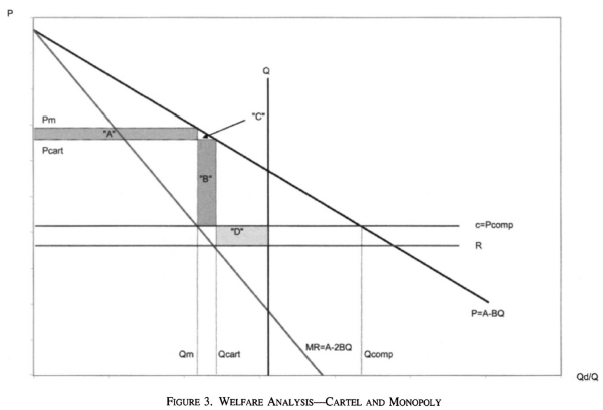
\includegraphics[scale=0.8]{l1_p1}} \\

 Under monopoly, marginal revenue equals marginal cost (in the figure, $MR = c$); under cartel, firms will fail to internalise the negative quantity externality they impose on each other when setting $q_i$, which will then result in (i) overproduction and (ii) lower prices ($MR = R$). \\
 Moving from cartel to monopoly implies the following changes in total welfare:
 \begin{itemize}
 	\item area A is a price rise, which constitutes a pure transfer from consumers to producers and as such is welfare neutral;
 	\item area B is a welfare loss (consumers buy less, firm does not sell);
 	\item area C is a deadweight loss;
 	\item area D is a welfare gain (firms lose less from exporting less at $r < mc$.)
 \end{itemize}
 so the total welfare change is D - B - C: whether moving to monopoly is welfare-improving is ambiguous.

\subsection{Estimation}
Roller and Steen estimate the following ADL(1,1) equation:
\begin{equation}
	p_t = \alpha_0 + \beta_0 q^D_t + \beta_1 q^D_{t-1} + \beta_2 z_t + \beta_3 z_{t-1} + \gamma p_{t-1} + \varepsilon_t
\end{equation}
recognising endogeneity, they instrument $q^D$ with world price $r$, which enters the cartel's quantity setting rule \eqref{cartelq} but is independent of domestic $\varepsilon_t$.
They then estimate long run elasticity as (at steady state $q_D$, $p$ values)
\begin{equation}
	\eta_{LR} \equiv \frac{1 - \gamma}{\beta_0 + \beta_1} \frac{q_D}{p} = -1.468
\end{equation}
which passes the litmus test of $|\eta| > 1$.
From Equation \eqref{firmmax} they then obtain marginal costs, which allow for counterfactual estimation of Cournot and monopoly outputs: it turns out that the cartel structure was so inefficient that the switch to monopoly led to large \textbf{welfare gains}, as elimination of exporter net losses outweighed the losses to consumers from higher price.

\section{Market Conduct}
\subsection{The Conduct Parameter}
Consider the following:
\begin{itemize}
	\item Under monopoly, $\frac{\partial \pi^M}{\partial q^M} = p_d'(q^M)q^M - p_s(q^M) - c'(q^M)=0$, i.e. $p_s(q^M) = c'(q^M) - p_d'(q^M)q^M $.
	\item In symmetric perfect competition with $N$ firms, $p_s(q^{PC}) = c'(q^{PC}/N)$.
	\item Under Cournot competition, the symmetric solution is $ p_s(q^{CC}) = c'(\frac{q^{CC}}{N}) - p'_d(q^{CC}) \underbrace{\frac{q^{CC}}{N}}_{q_i}$
\end{itemize}
All of these functions can be nested by a more general form
\begin{equation}
	\label{conduct}
	p_s(q) = c'(\frac{q}{N}) - \theta p'_d(q)q
\end{equation}
we call $\theta$ the \textbf{conduct parameter}.
Basically, a value $\hat{\theta}$ of $\theta$ implies that \textbf{an industry is behaving as if it was a Cournot oligopoly with $\frac{1}{\hat{\theta}}$ firms}: e.g. in perfect competition $\hat{\theta}=0$, consistent with perfect competition being equivalent to a $N\rightarrow \infty$ Cournot game.
The conduct parameter has a direct relationship with the Lerner index of industry market power:
\begin{equation}
\label{lerner}
	\mathcal{L} \equiv \frac{p - c'}{p} \overset{\eqref{conduct}}{=} \theta \frac{\partial p_d}{\partial q} \frac{q}{p}  \overset{\eqref{ownelas}}{\equiv}  \frac{\theta}{|\eta|}
\end{equation}

\subsection{Is the Conduct Parameter Identified? (Bresnahan, 1982)}

Let's parameterise Equation \eqref{conduct}: let inverse demand be
\begin{equation}
	\label{invd}
	p_d(q) = \alpha + \beta_1 q + \beta_2 q x + \beta_3 z + \varepsilon_d
\end{equation}
where $x$ is called ``\textbf{rotator}'' and $z$ is called ``shifter''. Also, let unobserved\footnote{We usually do not observe marginal cost; we parameterise it to substitute in the following.} marginal cost be (under $q_i = \frac{q}{N}$)
\begin{equation}
	\label{mceq}
	c'(q) = \gamma_0 + \gamma_1 q_i + \varepsilon_s =  \gamma_0 + \underbrace{\tilde{\gamma}_1}_{\tilde{\gamma}_1 = \frac{\gamma_1}{N}} q + \varepsilon_s
\end{equation}
then, plugging \eqref{invd} (which can be estimated) and \eqref{mceq} (which \textit{cannot}, in absence of marginal cost data) into \eqref{conduct},
\begin{equation}
	p_s(q) = \gamma_0 + \tilde{\gamma}_1 q - \theta (\beta_1 + \beta_2x) q + \epsilon_s \equiv  \gamma_0 + [\tilde{\gamma}_1 - \theta (\beta_1 + \beta_2x)] q + \epsilon_s
\end{equation}
Is $\theta$ identified? The answer ultimately depends on $\beta_2$:
\begin{itemize}
	\item If $\beta_2 = 0$, we have $p_s(q) = \gamma_0 +(\tilde{\gamma}_1 - \theta \beta_1) q+ \epsilon_s$, and it is ultimately impossible to distinguish conduct from the marginal cost parameter, even if we have $\hat{\beta}_1$.
	\item If $\beta_2 \neq 0$ instead, $q$ and $(\beta_1 + \beta_2x)q$ are not collinear because of the rotator, and the $\theta$ parameter can be identified as a nonlinear combination of $\beta_1$ and $\beta_2$ (conditional on estimates $\hat{\beta}_1, \hat{\beta}_2$ we have two unknowns, $\tilde{\gamma}_1$ and $\theta$, in two variables, $q$ and $qx$).
\end{itemize}
The intuition is that ``rotation'' of demand around the equilibrium price changes marginal revenue (= price for a monopolist), but it \textbf{does not affect a competitive firm}.
We need an external variable that does not affect valuation for the highest-valuation consumers (intercept fixed), but \textbf{changes willingness to pay for consumers with lower valuation}: in such a case, $P=MC$ would still hold under perfect competition, but under market power prices would change along exogenous demand shocks caused by the rotator.
The identification carries through to marginal cost parameters, which are not usually observed. \\
\textbf{Caveat}: Unsurprisingly, estimation of $\eqref{conduct}$ might yield biased measures of market power if the generating data does not fit this form (Corts, 1999).

\subsection{Estimating $\theta$ from Observed Marginal Cost}

Conditional on being able to observe the marginal cost $c'(q)$, we simply need an estimate of demand slope $p'_d(q)$ to invert Equation \eqref{conduct}:
\begin{equation}
	\theta = \frac{p - c'}{- p'_d(q)q}
\end{equation}
which yields an estimate that is independent of supply curve estimation, and is thus devoid of potential misspecification bias. Even if $\theta$ does not \textit{exactly} capture firm behaviour, it is still a useful market power index (recall $\theta \propto \mathcal{L}$ from equation \eqref{lerner}).

\section{Application: Genesove and Mullin (1998)}

Analysis of the sugar market, which was very concentrated up to the 1890 Sherman Act. Availability of reliable marginal cost data (from knowledge of the manufacturing process) makes computation of $\theta$ feasible with both the estimation and the rearrangement methods. \\
In particular, marginal cost of sugar is defined as
\vspace{-.25cm}
\begin{equation}
	mc = mc_0 + \kappa p_{raw}
\end{equation}
where $p_{raw}$ is the price of raw sugar, $\kappa$ is a known constant and $mc_0$ is set based on anti-trust data.

Assuming that\footnote{as one does} $p_d(q) = \alpha + \frac{1}{\beta}q$, we have $p'_d(q) = \frac{1}{\beta}$ and $q = \beta(p_d - \alpha)$. Plugging into Equation \eqref{conduct},
\begin{equation}
	p_s(q) = mc - \frac{\theta}{\beta}\beta(p_d - \alpha)
\end{equation}
which in equilibrium rearranges to
\begin{equation}
	p = \frac{mc + \theta \alpha}{1 + \theta}
\end{equation}
and using the marginal cost condition yields
\begin{equation}
	(1 + \theta) p - mc_0 - \kappa p_{raw} - \theta \alpha = 0
\end{equation}
given that we assume\footnote{as one does} the structure of the demand function, we can obtain an estimate of $\hat{\alpha}$, and then use a marginal cost shifter $z$ -- specifically the price of imported Cuban raw sugar -- to estimate $\theta$ from the following condition
\begin{equation}
	\mathbb{E}[(1 + \theta) p - mc_0 - \kappa p_{raw} - \theta \alpha | z] = 0
\end{equation}
which yields $\hat{\theta} =$ \textbf{0.038} (se. = 0.024) - \textbf{not significantly different from zero} (which recall is the $\theta$ for perfect competition). The rearrangement method yields instead a $\hat{\theta}$ of around \textbf{0.10}.
Interestingly, at the time $N = 6$, while the estimated conduct would suggest $N \geq 10$, so the industry seems to have behaved \textit{more competitively} than under Cournot; moreover, the discrepancy between estimated and calculated $\hat{\theta}$ is a further reminder of the potential consequences of model misspecification on conduct parameter estimation.


\end{document}
